\documentclass[10pt]{article}\usepackage[]{graphicx}\usepackage[]{color}
%% maxwidth is the original width if it is less than linewidth
%% otherwise use linewidth (to make sure the graphics do not exceed the margin)
\makeatletter
\def\maxwidth{ %
  \ifdim\Gin@nat@width>\linewidth
    \linewidth
  \else
    \Gin@nat@width
  \fi
}
\makeatother

\usepackage{Sweavel}


\usepackage{hyperref}
\usepackage{url}
\usepackage[a4paper]{geometry}
\usepackage{a4wide}
\usepackage{float}
\usepackage[english]{babel}
\usepackage[utf8]{inputenc}
\usepackage{csquotes}
\usepackage{amsmath}
\usepackage{amssymb}
\usepackage{xspace}
\usepackage[numbers]{natbib}
\bibliographystyle{unsrtnat}
\usepackage{subcaption}
\usepackage[font={small}]{caption}
\usepackage{booktabs}
\usepackage{listings}
\usepackage{cleveref}
\usepackage{lipsum}
\newcommand{\approxtext}[1]{\ensuremath{\stackrel{\text{#1}}{=}}}
\newcommand{\matr}[1]{\mathbf{#1}}
\newcommand{\partt}[2]{\ensuremath{\dfrac{\partial {#1}}{\partial {#2}}}}
\renewcommand{\d}[1]{\ensuremath{\operatorname{d}\!{#1}}} % non-italized differentials
\newcommand{\h}[0]{\ensuremath{\hbar}} % hbar
\def\changemargin#1#2{\list{}{\rightmargin#2\leftmargin#1}\item[]}
\let\endchangemargin=\endlist 
\usepackage{amsthm}
\theoremstyle{plain}
\renewcommand{\theequation}{\thesection.\arabic{equation}}
\def\changemargin#1#2{\list{}{\rightmargin#2\leftmargin#1}\item[]}
\let\endchangemargin=\endlist    
\usepackage{xcolor}
\definecolor{Red}{rgb}{0.7,0,0}
\definecolor{Blue}{rgb}{0,0,0.8}
\usepackage{verbatim}
\def\changemargin#1#2{\list{}{\rightmargin#2\leftmargin#1}\item[]}
\let\endchangemargin=\endlist
\addtolength{\oddsidemargin}{-.35in}
\addtolength{\evensidemargin}{-.35in}
\addtolength{\textwidth}{.7in}
\usepackage{multicol}

% Stephen's stuff
\newcommand{\R}{\texttt{R}}
\newcommand{\Rfunction}[1]{{\texttt{#1}}}
\newcommand{\Robject}[1]{{\texttt{#1}}}
\newcommand{\Rpackage}[1]{{\mbox{\normalfont\textsf{#1}}}}
\usepackage{xcolor}
\definecolor{Red}{rgb}{0.7,0,0}
\definecolor{Blue}{rgb}{0,0,0.8}
\hypersetup{%
pdfusetitle,
bookmarks = {true},
bookmarksnumbered = {true},
bookmarksopen = {true},
bookmarksopenlevel = 2,
unicode = {true},
breaklinks = {false},
hyperindex = {true},
colorlinks = {true},
linktocpage = {true},
plainpages = {false},
linkcolor = {Blue},
citecolor = {Blue},
urlcolor = {Red},
pdfstartview = {Fit},
pdfpagemode = {UseOutlines},
pdfview = {XYZ null null null}
}
%% Listings
\lstset{ 
language=R,                     % the language of the code
basicstyle=\footnotesize,       % the size of the fonts that are used for the code
numbers=left,                   % where to put the line-numbers
numberstyle=\tiny\color{gray},  % the style that is used for the line-numbers
stepnumber=1,                   % the step between two line-numbers. If it's 1, each line will be numbered
numbersep=5pt,                  % how far the line-numbers are from the code
backgroundcolor=\color{white},  % choose the background color. You must add \usepackage{color}
showspaces=false,               % show spaces adding particular underscores
showstringspaces=false,         % underline spaces within strings
showtabs=false,                 % show tabs within strings adding particular underscores
rulecolor=\color{black},        % if not set, the frame-color may be changed on line-breaks within not-black text (e.g. commens (green here))
tabsize=2,                      % sets default tabsize to 2 spaces
captionpos=b,                   % sets the caption-position to bottom
breaklines=true,                % sets automatic line breaking
breakatwhitespace=false,        % sets if automatic breaks should only happen at whitespace
title=\lstname,                 % show the filename of files included with \lstinputlisting;
% also try caption instead of title
keywordstyle=\color{Blue},      % keyword style
commentstyle=\color{orange},    % comment style
stringstyle=\color{Red},        % string literal style
escapeinside={\%*}{*)},         % if you want to add a comment within your code
morekeywords={*,...}            % if you want to add more keywords to the set
} 

%%% Document specific
\newcommand{\course}{Population Genetics}
\newcommand{\ass}{2}
\newcommand{\term}{Lent term 2017}

% Commands for this report
\newcommand{\ABBA}{\texttt{ABBA}\xspace}
\newcommand{\BABA}{\texttt{BABA}\xspace}
\newcommand{\A}{\texttt{A}\xspace}
\newcommand{\B}{\texttt{B}\xspace}
\renewcommand{\C}{\texttt{C}\xspace}
\newcommand{\D}{\texttt{D}\xspace}

%%% Title page
\title{
  \bf \course: Assignment \ass \\[1em]
  \small{University of Cambridge}
}

\author{Henrik Åhl}
\date{\today}
\renewcommand{\textfraction}{0.05}
\renewcommand{\topfraction}{0.8}
\renewcommand{\bottomfraction}{0.8}
\renewcommand{\floatpagefraction}{0.75}

%%% Actual document
\begin{document}
\date{\today}
\maketitle
\setcounter{page}{1}


\maketitle

\begin{multicols*}{2}
\section*{Preface}
This is an assignment report in connection to the \textit{\course}
module in the Computational Biology course at the University of Cambridge,
\term. All related code is as of \date{\today} available through a
Github repository by contacting \href{mailto:hpa22@cam.ac.uk}{hpa22@cam.ac.uk}.

\section*{Exercises}
\paragraph*{1}
Under the population size of $N \sim 10^7$, we get that the variance will be relatively low, and therefore not be a determining factor for the development of the allele frequency. We thus get the equation $$q(t) = q_{0} \dfrac{e^{\sigma t}}{1 - q_0 + q_0 e^{\sigma t}}$$ as an estimator for the development of $q$. Our likelihood function for a model $\mathcal M$ can then be describes as $$ \mathcal L = \sum_k \log \dfrac{N!}{n_A(t_k)! n_a(t_k)!}q_A(t_k)^{n_A(t_k)}q_a(t_k)^{n_a(t_k)},$$ where the $n$'s are our observations, and the $q$'s our model predictions, compared to some number of total observations $N$, which in our case is the number of reads. We optimise the log-likelihood using L-BFGS-B optimisation the \R~function \texttt{stats4::mle}, having set $q$ bounded at 0 and 1. 



\begin{Schunk}
\begin{figure}[H]

{\centering 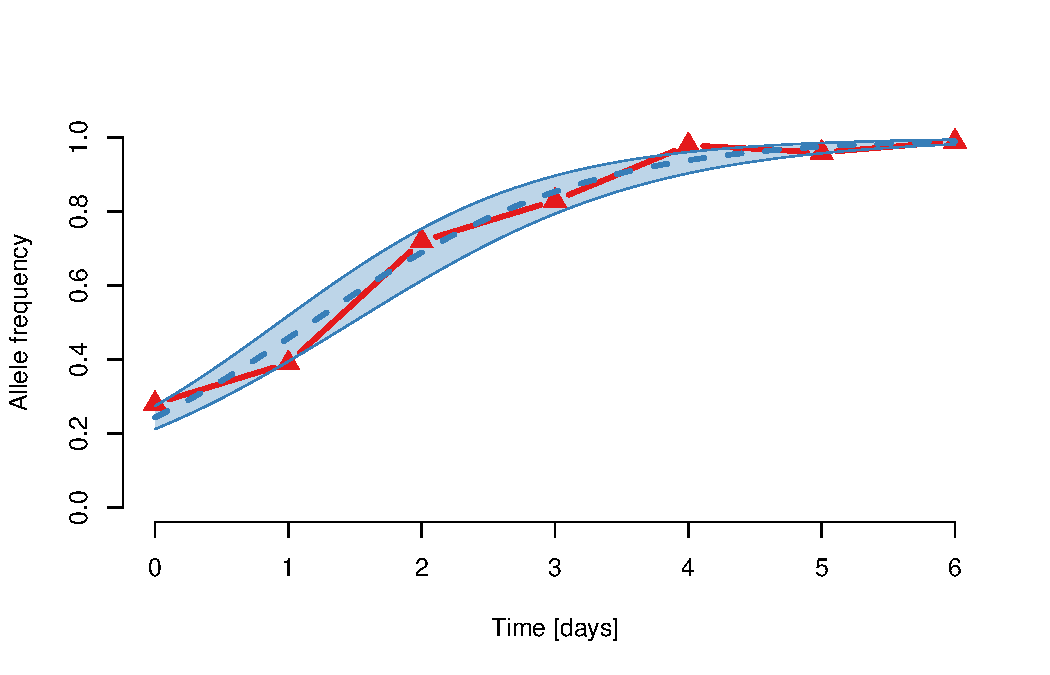
\includegraphics[width=\maxwidth]{figure/twocolumn-1_inference-1} 

}

\caption[Allele development as given by data (red) and model]{Allele development as given by data (red) and model. The shaded area denotes the 95~\% confidence interval of the optimisation.}\label{fig:1_inference}
\end{figure}
\end{Schunk}
The results of the optimisation can be seen in \cref{fig:1_inference}, where the shaded area signifies the range of the standard error.  Compare this to our found optimal values of 
$q_0 = 0.24 \pm 0.03$ and
$\sigma = 0.97 \pm 0.08$

\Cref{fig:1_surface} shows the negative log-likelihood surface for $\sigma$ and $q$. Due to the growth rate of the log-likelihood, some configurations give rise to numerical errors, as shown by the white surface in the figure. Note in particular the darker shaded area, which signifies the most likely parameter configurations. 
\begin{Schunk}
\begin{figure}[H]

{\centering 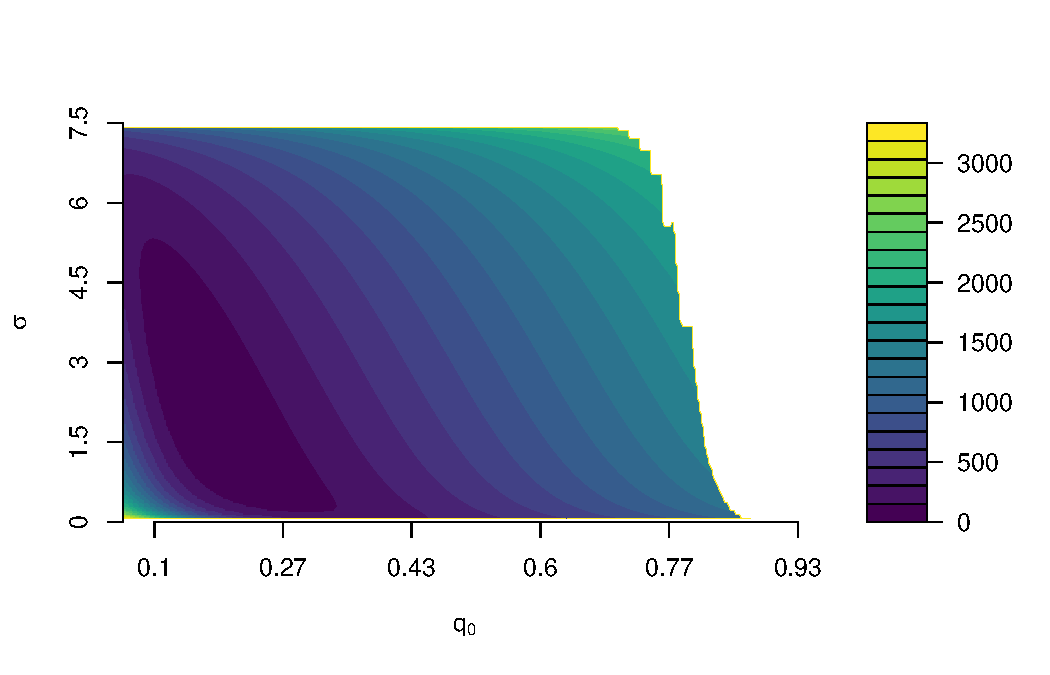
\includegraphics[width=\maxwidth]{figure/twocolumn-1_surface-1} 

}

\caption[Contour plot of the negative log-likelihood surface for different parameter configurations]{Contour plot of the negative log-likelihood surface for different parameter configurations. Note how our optimised parameters indeed fall inside the optimum.}\label{fig:1_surface}
\end{figure}
\end{Schunk}

\paragraph*{2}
We download the \textit{Optimist} package according to instructions. For all of our investigations, we use a seed value of 2. For our simulations with this, we get a log-likelihood of $-92.5714$, without any variance. 



When instead perform a more thorough optimisation, we get the results seen in \cref{fig:2_fitted_curves} for our three cases. We can visually note that two and three mutations seem to fit better with the data. When observing the average log-likelihoods, we can also note that increasing from two to three mutations does not seem to produce better results, hinting at redundancy in the number of free parameters.  Looking at the AIC and BIC scores in \cref{fig:2_aic_bic}, we see that two beneficial mutations indeed give us the best model for the data. 

However, we must be aware of that because we have such little data, with few data points that have been manually acquired. We therefore have a high uncertainty in the data itself that must be considered. Possibly, this is what causes the majority of our observed variance, since the population size suggests that the fluctuations should be minor. With the error present, it might prove useful to fit a model with drift in order to account for the additional variability. Directly attempting to attain estimates of the acquisition errors would of course also be preferable, in case there is no possibility of performing repeated trials. 

\begin{Schunk}
\begin{figure}[H]

{\centering 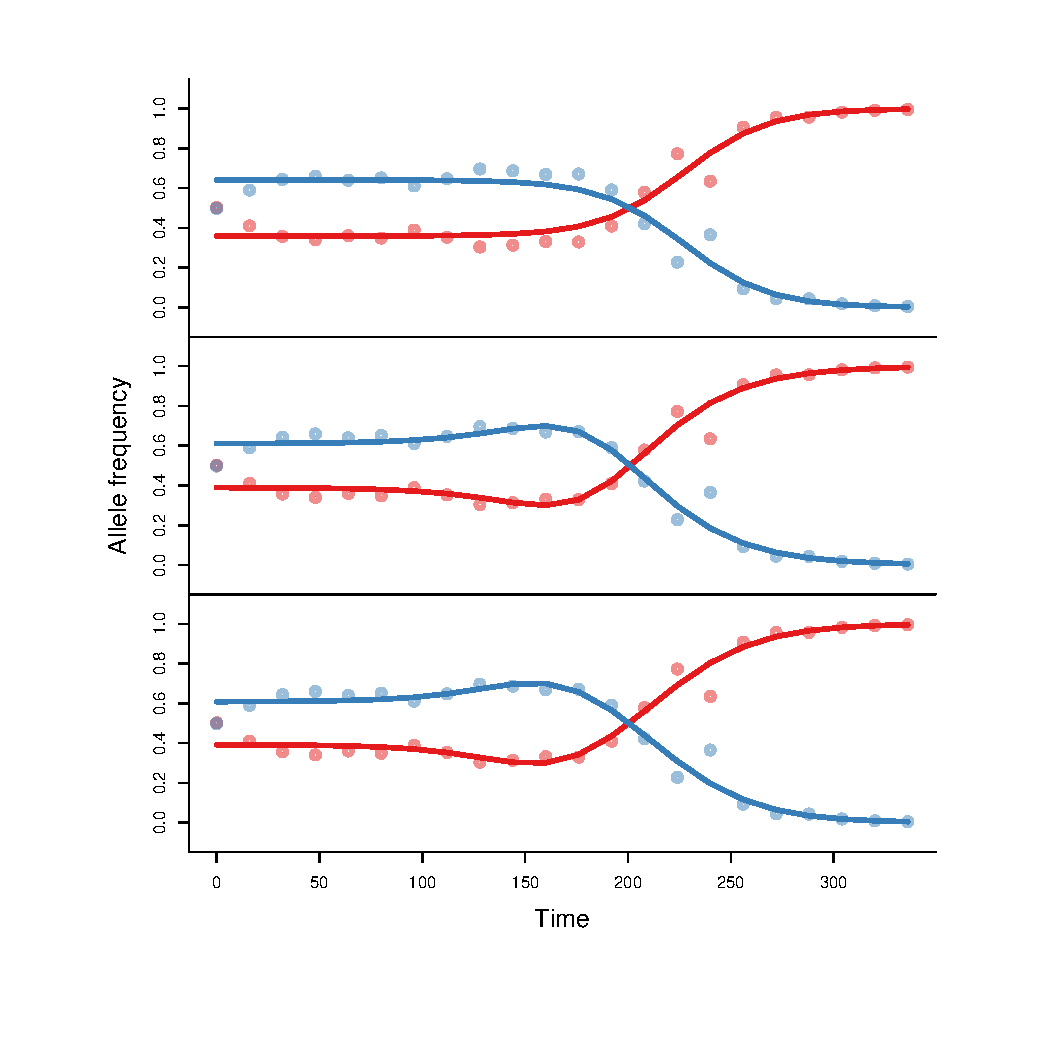
\includegraphics[width=\maxwidth]{figure/twocolumn-2_fitted_curves-1} 

}

\caption[Fitted curves under models with one, two, or three mutations respectively]{Fitted curves under models with one, two, or three mutations respectively.}\label{fig:2_fitted_curves}
\end{figure}
\end{Schunk}

\begin{Schunk}
\begin{figure}[H]

{\centering 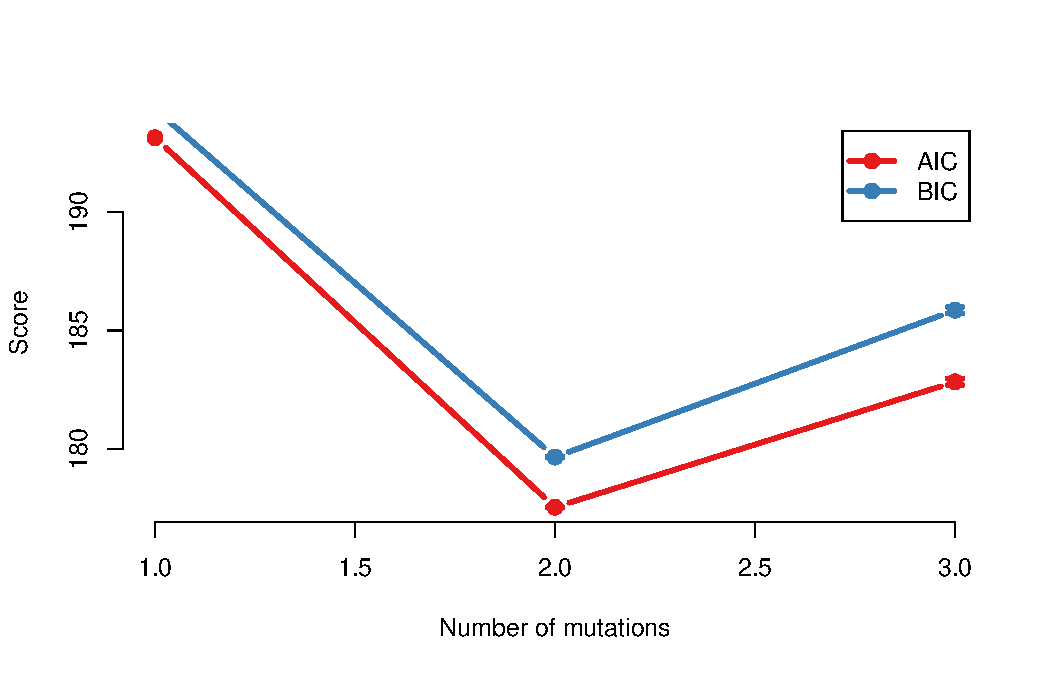
\includegraphics[width=\maxwidth]{figure/twocolumn-2_aic_bic-1} 

}

\caption[AIC and BIC scores, with errorbars corresponding to the standard error, for the 10 optimisations]{AIC and BIC scores, with errorbars corresponding to the standard error, for the 10 optimisations. Two mutations consistently performs the best, with significance.}\label{fig:2_aic_bic}
\end{figure}
\end{Schunk}

%e
Antibiotic resistance can the achieved through many different ways, and depends largely on the type of organism, the population size, and the generation length. One example could be the accumulation of single-nucleotide polymorphisms which in various ways can affect the function of the antibiotic. A common inactivation method for several antibiotics is enzymatic inactivation through hydrolysis, which can occur due to SNP's increasing the likelihood of such events taking place~\cite{martinez2000mutation}. Several antibiotics, such as quinolone cipofloxacin, targets parts of the bacterial genome itself in order to prevent replication. Like antibiotics themselves can be target indirectly through mutations, resistance can also arise due to mutations altering the targets of the antibiotics~\cite{truong1997novel}. A third option for mutations to be beneficial is by having them alter the membrane selectivity such that the antibiotics are unable to reach their molecular targets~\cite{delcour2009outer}. 

All these changes induce a selective pressure towards keeping the mutation within the population. These can thereafter progress through direct inheritance, as well as thorugh horizontal transfer. It might also be that the antibiotics wipe out most of the population aside for the select few who have acquired beneficial mutations, whereafter these instead can replicate successfully and establish a completely new population consisting primarily of resistant cells~\cite{martinez2000mutation}.

% Windows, D-values similar
\paragraph*{3}

Using the data provided, we get the resulting values of $D = -0.12, n_{abba} = 25$ and $n_{baba} = 32$. We clearly have a slightly higher number of \ABBA than \BABA, and therefore some inferred introgression between \A and \C. 

Calculating a p-value for the D-value observed, we get a result of $0.43$, saying we cannot reject the null-hypothesis. However, this assumes that the sites are independent of each other, which we know they are not, and we must go to additional lengths to ensure ourselves of the significance. In order to do this, we calculate the allele frequencies, whose first few rows indeed correspond with the example supplied, apart from an apparent typo in the instructions.

When instead using the allele frequencies, we now get a result of $D = -0.19$, i.e.\ higher than before now that more data is incorporated. Likewise, our p-value is significantly lower, reaching $p = 0.0017278$ In this scenario, our results are indeed significant, and we can reject the null-hypothesis. 

Given the figure for the linkage disequilibirium between populations \A and \B, we see that there is indeed significant short-range interactions in both of the populations. We look at the distributions between minimum distances for our SNPs, we get \cref{fig:3_distances} and see that the distribution pans of quickly after a distance of ca 20000. Most SNPs are thus in this high-correlated zone that we see before the bend in our instruction figure. 

\begin{Schunk}
\begin{figure}[H]

{\centering 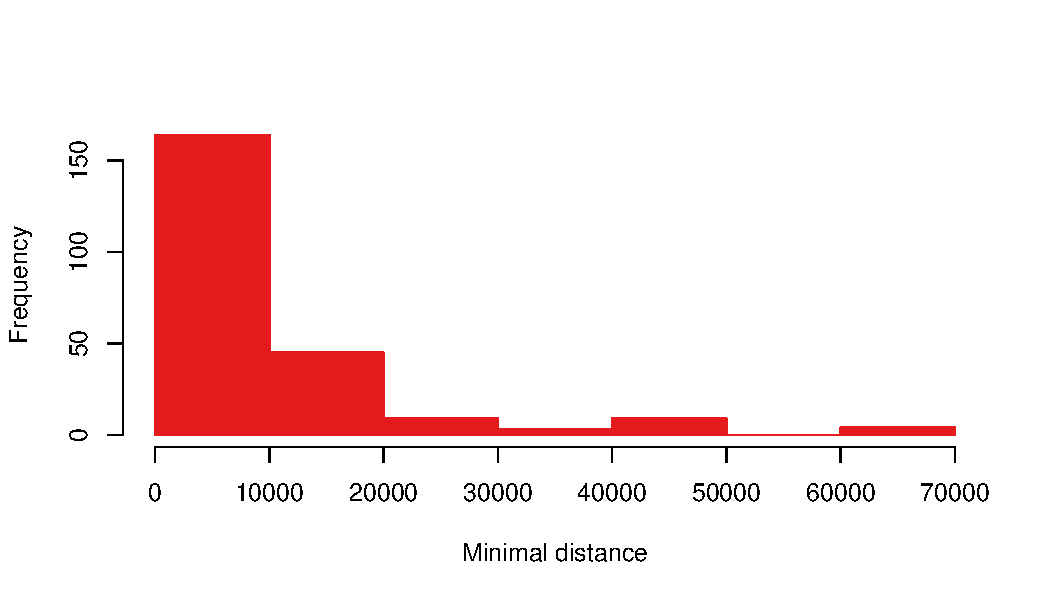
\includegraphics[width=\maxwidth]{figure/twocolumn-3_distances-1} 

}

\caption[Minimum neighbour distance distribution]{Minimum neighbour distance distribution. Apparently, most SNPs are within 20000-30000 basepairs of their closest neighbour.}\label{fig:3_distances}
\end{figure}
\end{Schunk}



We want too choose the jackknife when the correlation has panned out, and thus take it to be at a distance of 30000. Separating our data into chunks of this size and perform the analysis, we now get a p-value of $0.0062384$, slightly worse than the  leave-one-out cross-validation case.

In the last figure of the assignment, population \B appears to be affiliated with a slightly higher short-interaction density, and lower intermediate-interaction density. Since we know that populations which diverged long ago should display high short-range correlation, we can infer that \B diverged from \C earlier than \A. Comparing to above, where we note introgression between \A and \C, the results can indeed be said to be consistent. 

\bibliography{references}
\end{multicols*}

\newpage
\onecolumn
  \appendix
\section{Code}
   \lstinputlisting{../code/exc1.R}
   \lstinputlisting{../code/exc2.R}
   \lstinputlisting{../code/exc3.R}
\end{document}
